%------------------------------------------
% Example: image registration and stitching
%------------------------------------------

\section*{Example: image registration and stitching}
  \label{sec:example-image-registration-and-stitching}

  This section gives a step-by-step outline of how to perform panorama stitching using the primitives found in scikit-image. The full source code is at \url{https://github.com/scikit-image/scikit-image-demos}.

  \subsection{Data loading}
    \label{sub:data_loading}

    The ``ImageCollection'' class provides an easy way of representing multiple images on disk. For efficiency, images are not read until accessed.

    \begin{pyverbatim}
      from skimage import io
      ic = io.ImageCollection('data/*')
    \end{pyverbatim}

    Figure~\ref{fig:petra} shows the Petra dataset, which displays the same facade from two different angles. For this demonstration, we will estimate a projective transformation that relates the two images. Since the outer parts of these photographs do not comform well to such a model, we select only the central parts. To further speed up the demonstration, images are downscaled to 25\% of their original size.

    \begin{pyverbatim}
      from skimage.color import rgb2gray
      from skimage import transform

      image0 = rgb2gray(ic[0][:, 500:500+1987, :])
      image1 = rgb2gray(ic[1][:, 500:500+1987, :])

      image0 = transform.rescale(image0, 0.25)
      image1 = transform.rescale(image1, 0.25)
    \end{pyverbatim}

  \subsection{Feature detection and matching}
    \label{sub:feature_detection_and_matching}

    ``Oriented FAST and rotated BRIEF'' (ORB) features \citep{ORB} are detected in both images. Each feature yields a binary descriptor; those are used to find the putative matches shown in Figure~\ref{fig:putativematches}.

    \begin{pyverbatim}
      from skimage.feature import ORB, match_descriptors

      orb = ORB(n_keypoints=1000, fast_threshold=0.05)

      orb.detect_and_extract(image0)
      keypoints1 = orb.keypoints
      descriptors1 = orb.descriptors

      orb.detect_and_extract(image1)
      keypoints2 = orb.keypoints
      descriptors2 = orb.descriptors

      matches12 = match_descriptors(descriptors1,
                                    descriptors2,
                                    cross_check=True)
    \end{pyverbatim}

  \subsection{Transform estimation}
    \label{sub:transform_estimation}

    To filter the matches, we apply RANdom SAmple Consensus (RANSAC) \citep{ransac}, a common method for outlier rejection. This iterative process estimates transformation models based on randomly chosen subsets of matches, finally selecting the model which corresponds best with the majority of matches. The new matches are shown in Figure~\ref{fig:matchesfiltered}.

    \begin{pyverbatim}
      from skimage.measure import ransac

      # Select keypoints from the source (image to be
      # registered) and target (reference image).

      src = keypoints2[matches12[:, 1]][:, ::-1]
      dst = keypoints1[matches12[:, 0]][:, ::-1]

      model_robust, inliers = \
          ransac((src, dst), ProjectiveTransform,
                 min_samples=4, residual_threshold=2)
    \end{pyverbatim}

  \subsection{Warping}
    \label{sub:warping}

    Next, we produce the panorama itself. The first step is to find the shape of the output image by considering the extents of all warped images.

    \begin{pyverbatim}
      r, c = image1.shape[:2]

      # Note that transformations take coordinates in
      # (x, y) format, not (row, column), in order to be
      # consistent with most literature.
      corners = np.array([[0, 0],
                          [0, r],
                          [c, 0],
                          [c, r]])

      # Warp the image corners to their new positions.
      warped_corners = model_robust(corners)

      # Find the extents of both the reference image and
      # the warped target image.
      all_corners = np.vstack((warped_corners, corners))

      corner_min = np.min(all_corners, axis=0)
      corner_max = np.max(all_corners, axis=0)

      output_shape = (corner_max - corner_min)
      output_shape += np.abs(corner_min)
      output_shape = output_shape[::-1]
    \end{pyverbatim}

    The images are now warped according to the estimated transformation model. Values outside the input images are set to -1 to distinguish the ``background''.

    A shift is added to ensure that both images are visible in their entirety. Note that \texttt{warp} takes the \textit{inverse} mapping as input.

    \begin{pyverbatim}
      from skimage.color import gray2rgb
      from skimage.exposure import rescale_intensity
      from skimage.transform import warp
      from skimage.transform import SimilarityTransform

      offset = SimilarityTransform(translation=-corner_min)

      image0_ = warp(image0, offset.inverse,
                     output_shape=output_shape, cval=-1)

      image1_ = warp(image1, (offset + model_robust).inverse,
                     output_shape=output_shape, cval=-1)
    \end{pyverbatim}

    An alpha channel is added to the warped images before merging them into a single image:

    \begin{pyverbatim}
      def add_alpha(image, background=-1):
          """Add an alpha layer to the image.

          The alpha layer is set to 1 for foreground
          and 0 for background.
          """
          rgb = gray2rgb(image)
          alpha = (image != background)
          return np.dstack((rgb, alpha))

      image0_alpha = add_alpha(image0_)
      image1_alpha = add_alpha(image1_)

      merged = (image0_alpha + image1_alpha)
      alpha = merged[..., 3]

      # The summed alpha layers give us an indication of
      # how many images were combined to make up each
      # pixel.  Divide by the number of images to get
      # an average.
      merged /= np.maximum(alpha, 1)[..., np.newaxis]
    \end{pyverbatim}

    The merged image is shown in Figure~\ref{fig:merged}. Note that, while the columns are well aligned, the color intensities at the boundaries are not well matched.

  % Combine multiple pano sub-figures elegantly with LaTeX
  %----------------------
% Panorama multi-figure
%----------------------

\begin{figure}
\begin{frame}{}

% Left side of figure: stack of 4 images showing progressive steps
\begin{minipage}{.49\textwidth}

  % Original Petra images
  \begin{subfigure}{\linewidth}
    \centering
    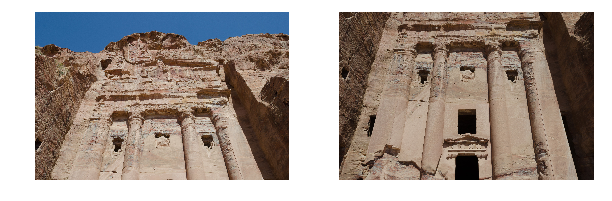
\includegraphics[width=\linewidth]{pano_4_0.png}
    \caption{Petra images\label{fig:petra}}
  \end{subfigure} \\ [0.5ex]  % Small vertical pad

  % Unfiltered ORB features
  \begin{subfigure}{\linewidth}
    \centering
    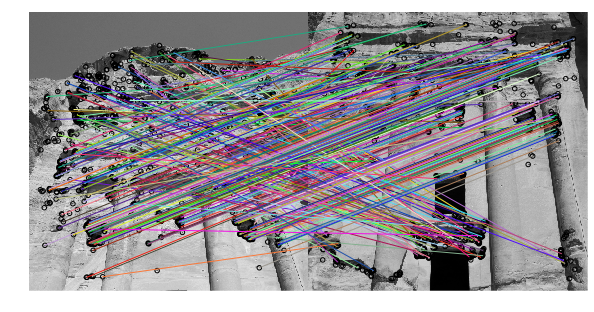
\includegraphics[width=\linewidth]{pano_11_1.png}
    \caption{ORB binary features\label{fig:putativematches}}
  \end{subfigure} \\ [0.5ex]  % Small vertical pad

  % ORB features after RANSAC padding
  \begin{subfigure}{\linewidth}
    \centering
    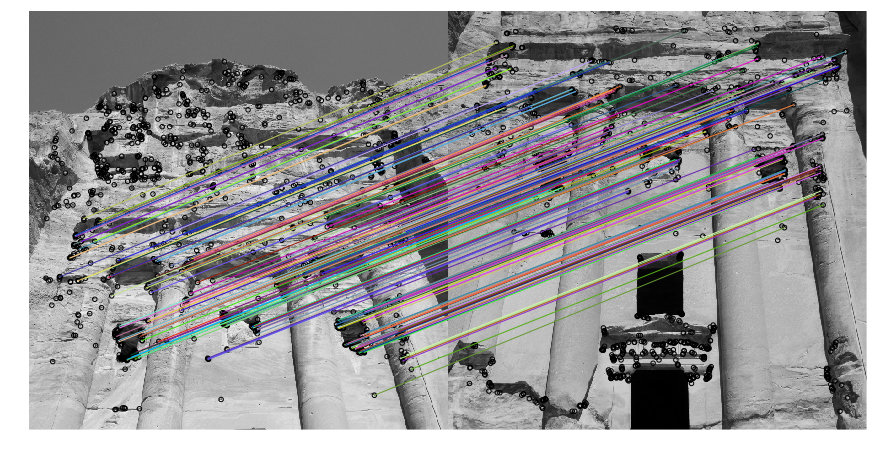
\includegraphics[width=\linewidth]{pano_15_1.png}
    \caption{RANSAC-filtered features\label{fig:matchesfiltered}}
  \end{subfigure} \\ [0.5ex]  % Small vertical pad

  % Correct orientation & simple averaged combination
  \begin{subfigure}{\linewidth}
    \centering
    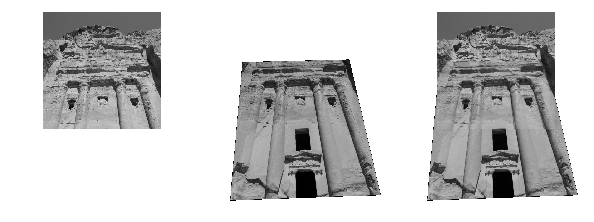
\includegraphics[width=\linewidth]{pano_23_0.png}
    \caption{Warped \& positioned\label{fig:merged}}
  \end{subfigure}
\end{minipage}%
% Right side of figure: Final Enblend result
\begin{minipage}{.5\textwidth}
  \begin{subfigure}{\linewidth}
    \centering
    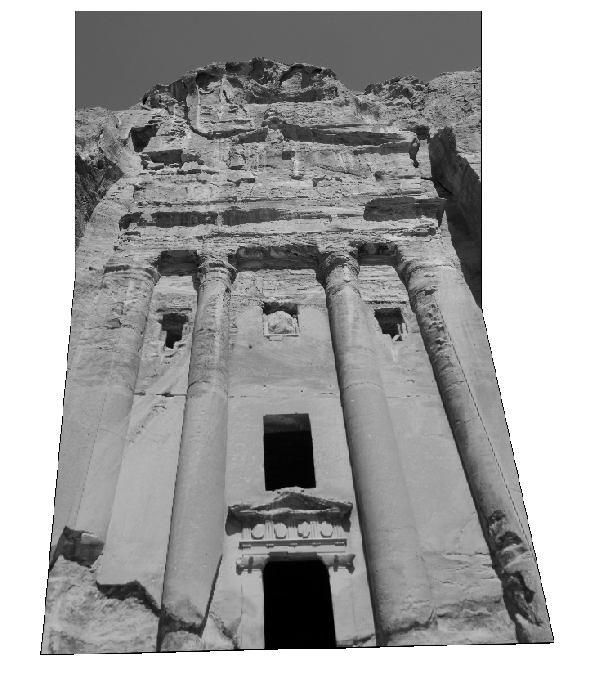
\includegraphics[width=\linewidth]{pano_28_0.png}
    \caption{Final result, combined with Enblend\label{fig:pano}}
  \end{subfigure}
\end{minipage}%
\end{frame}

\caption{An example application of scikit-image: image registration and warping to combine overlapping images. (\subref{fig:petra}): Photographs taken in Petra, Jordan by François Malan. License: CC-BY. (\subref{fig:putativematches}): Putative matches computed from ORB binary features. (\subref{fig:matchesfiltered}): Matches filtered using RANSAC. (\subref{fig:merged}): The second input frame (\textit{middle}) is warped to align with the first input frame (\textit{left}), yielding the averaged image shown on the right. (\subref{fig:pano}): The final panorama image, registered and warped using scikit-image, blended with Enblend.\label{fig:pano_overall}}

\end{figure}

  \subsection{Blending}
    \label{sub:blending}

    To blend images smoothly we make use of the open source package Enblend \citep{Enblend}, which in turn employs multi-resolution splines and Laplacian pyramids \citep{burt_adelson_0,burt_adelson_1}. The final panorama is shown in Figure~\ref{fig:pano}.
